\documentclass[sigconf]{acmart}

\usepackage{graphicx}
\usepackage{hyperref}
\usepackage{todonotes}

%\usepackage{endfloat}
%\renewcommand{\efloatseparator}{\mbox{}} % no new page between figures

\usepackage{booktabs} % For formal tables

\settopmatter{printacmref=false} % Removes citation information below abstract
\renewcommand\footnotetextcopyrightpermission[1]{} % removes footnote with conference information in first column
\pagestyle{plain} % removes running headers


\newcommand{\TODO}[1]{\todo[inline]{#1}}
\newcommand{\DONE}[1]{DONE: \todo[inline,color=green!30]{#1}}


\begin{document}
\title{Mapping the Social Network of Opioid Misuse on Twitter}


\author{Liz Supinski, Nandita Sathe, and Sean M. Shiverick}
\affiliation{%
  \institution{Indiana University-Bloomington}
  \institution{ILS-Z639: Social Media Mining - Spring 2018}
  \institution{Final Project Report: Group 1}
}
\email{smshiver@indiana.edu}

% The default list of authors is too long for headers}
\renewcommand{\shortauthors}{Supinski, Sathe, Shiverick}


\begin{abstract}
This paper provides a sample of a \LaTeX\ document which conforms, somewhat 
loosely, to the formatting guidelines for ACM SIG Proceedings.
\end{abstract}

\keywords{Infodemiology, Prescription Opioids, Opioid Misuse, Social Media 
Mining}

\maketitle


%%%%%%%%%%%%%%%%%%%%%%%%%%%%%%%%%%%%%%%%%%%%%%%%%%%%%%%%%%%%%%%%%%%%%%%%%%%%%%%%
\section{Introduction}

Over the past two decades, prescription opioid abuse and addiction in the U.S. 
has become a health crisis of epidemic proportion. Since 1999, the number of 
overdose deaths from prescription opioids, such as oxycodone and hydrocodone, 
has more than quadrupled \cite{nida18, cdc18}. Social media media mining (SMM) 
has been used to address public health concerns through ``infodemiology'' and 
``toxicovigilance'', which involves informatics for purposes of epidemiology, 
including strategies for monitoring patterns and prevalence of medication abuse 
\cite{eysenbach09, sarker16}. For example, researchers have tracked the outbreak 
of flu epidemics using internet searches and Twitter posts 
\cite{culotta10, paul14, lazer14}. Twitter data has also been used to track 
the expression of migraine headaches \cite{nascimento14}, detect misuse 
and abuse of prescription opioids \cite{sarker16, chary17, dzierak17}, and 
monitor illegal online sales of prescription opioids \cite{mackey17}. 
The relationship between Twitter posts and health outcomes is largely 
correlational, yet some research suggests that discussion of opioid misuse 
on Twitter may provide reinforcement for actual misuse of opioids 
\cite{hanson13}. Additional evidence would help to clarify the social network 
of Twitter users and the contexts of prescription opioid misuse. 

This project seeks to examine the relations among social media users posting 
content related to the misuse of prescription opioids (MUPO). Mapping social 
media content related to prescription opioid use may help detect individuals 
at risk for misusing prescription opioids, and identify factors related to 
opioid addiction. The main goal of this project is to map the social network
of prescription opioid misuse on Twitter. This proposal outlines several steps 
toward accomplishing this goal, which include: (a) Textual analysis of Twitter 
posts related to prescription opioid misuse, (b) Visualization of the 
geospatial location of Twitter users who post content on MUPO, and (c) Analysis 
of the social network of Twitter users who tweet about the MUPO. 

\subsection{Research Questions} 
\begin{enumerate}
    \item \emph{Can opioid misuse be detected by Twitter posts?} 
    \item \emph{Can the geographic location of opioid misuse be mapped 
    from Twitter posts?} 
    \item \emph{Can the social network of opioid misuse be mapped from 
    Twitter users?}  
\end{enumerate}

%%%%%%%%%%%%%%%%%%%%%%%%%%%%%%%%%%%%%%%%%%%%%%%%%%%%%%%%%%%%%%%%%%%%%%%%%%%%%%%%
\section{Literature Review} 

The misuse and abuse of opioids in the U.S. is a crisis with serious public 
health consequences. In 2015, an estimated 2 million Americans suffered from 
substance use disorders related to prescription opioid pain relievers 
\cite{nida18, cdc18}. Of patients legitimately prescribed opioids for chronic 
pain, between 21 to 29 percent misused them, 8 to 12 percent developed an 
opioid use disorder, and approximately 4 to 6 percent transitioned to heroin 
\cite{vowles15, carlson16}. Mobile health applications that monitor medication 
consumption have been developed to detect potential medication abuse 
\cite{varshney13}.

The field of infodemiology, broadly considered as the analysis of internet-
sourced health data for public health research, is still in its infancy. One 
of the best known infodemiological successes is the forecast of flu outbreaks 
by analyzing the correlation between the frequency of flu-related Twitter posts 
and official reports of influenza-like-illness from the CDC \cite{culotta10, 
paul14}. This research suggests that Twitter data can supplement official 
reports by providing information about the spread of flu 1 to 2 weeks earlier 
than the CDC-ILI. Because pharmaceutical manufacturers are obliged to monitor 
the safety of their drugs both before and after their release into the market,
a field known as ``pharmacovigilance'', the tools of infodemiology were quickly 
taken up in this field. Sarker and colleagues (2016) provide a methodological 
review studies using social media for pharmacovigilance, in which they point 
out that most studies rely on supervised learning with expert medical annotation 
of social media data \cite{sarker16}. 

In the area of prescription opioid misuse (MUPO), several works stand out. 
Chary and colleagues estimated misuse of prescription opioids from tweets, 
successfully detecting the incidence of tweets indicating opioid misuse with 
geographic incidence of opioid misuse as documented by the National Survey 
on Drug Use and Health (NSDUH) \cite{chary17}. This study used a customized 
version of Jiang-Conrath similarity algorithm \cite{jiang97} to determine the 
``kernal-weighted semantic distance'' between tweets and then used k-means 
clustering to separate tweets in opioid-misuse and non-opioid misuse 
categories. In a different study, Sarker et al. came up with a supervised 
classification technique to distinguish posts suggesting MUPO from non-MUPO 
posts \cite{sarker15}. Sarker and Gonzalez (2017) extended this work to present 
corpi for mining drug-related knowledge from Twitter using the \emph{word2vec} 
tool to train shallow neural networks with two layers \cite{sarker17} They have 
continued to enhance these models since publication, and made their trained 
models available to researchers online 
(\url{https://data.mendeley.com/datasets/dwr4xn8kcv/3}). 
These models can be used for natural language processing using the 
\emph{gensim} python library.

%%%%%%%%%%%%%%%%%%%%%%%%%%%%%%%%%%%%%%%%%%%%%%%%%%%%%%%%%%%%%%%%%%%%%%%%%%%%%%%%

Correlating twitter behavior with public health data requires that the twitter 
data be tied to geographic locations. Twitter geolocation is disabled by 
default and only a small number of users choose to enable it. It is estimated 
that only about 2 percent of tweets include geographic metadata, with the 
same prevalence found for GPS-tagged data \cite{chary17, leetaru13}. 
Chary and colleagues used a software package called \emph{Carmen} to geolocate 
tweets without geodata. Carmen is a library for geolocating tweets, available 
in both Java and Python implementations which, given a tweet, will return 
Location objects that represent a physical location \cite{dredze13}. Carmen 
infers structured location information (country, state, county, city) using 
geocoordinates (if available) and and user profile information, but not tweet 
content. In an early paper on use of Twitter to explore health-related topics, 
Prier and colleagues used the Twitter search API parameter to retrieve tweets 
on a state-by-state basis \cite{prier11}. Twitter geosearch method is 
proprietary, but the Twitter search API documentation suggests a combination 
of device/gps coordinates, user provided profile location, and network/IP 
address are probably used to location to determine tweets that fit within 
the geocode search parameter \cite{twitterGet}.

%%%%%%%%%%%%%%%%%%%%%%%%%%%%%%%%%%%%%%%%%%%%%%%%%%%%%%%%%%%%%%%%%%%%%%%%%%%%%%%%

Like other behaviors, opioid misuse may spread by social contact. Spreading 
or diffusion of contagious disease occurs within contact networks of direct 
person-to-person interaction or other indirect pathways \cite{pastor01}. In 
the case of opioids, rather than describing persons as infected or uninfected, 
people may be considered as more or less susceptible to misuse, dependence, and 
addiction, depending on individual and environmental factors \cite{volkow14}. 
Furthermore, the structure of the contact network can influence epidemic 
spreading \cite{watts98}, as the \emph{small-world} property of many networks 
reveals that the distance between nodes is reduced by the pattern of 
connections within the network. In a social network any two random acquaintances 
may be connected, on average, by five to six intermediaries \cite{travers69}. 
Contact networks of drug use may have small-world properties as a few highly 
connected nodes can rapidly transmit contagion (i.e., drugs) throughout the 
network \cite{shaham03}. For simple contagion, weak ties among acquaintances or 
infrequent associations can also provide shortcuts between distant nodes within 
the network \cite{granovetter73}, and facilitate the spread of contagion or 
drug use. Social media research suggests that discussion of prescription drug 
abuse on Twitter is potentially reinforcing of medication abuse within an 
online social network \cite{hanson13}. Experimental evidence has also shown 
the structure of an artificially constructed online community influenced the 
spreading of behavior, as individuals who received reinforcement from multiple 
connections within their social network were more likely to adopt a health
behavior \cite{centola10}. Behavior also spreads farther and faster through 
small-world networks that are clustered and latticed than random networks.

%%%%%%%%%%%%%%%%%%%%%%%%%%%%%%%%%%%%%%%%%%%%%%%%%%%%%%%%%%%%%%%%%%%%%%%%%%%%%%%%

\subsection{Gap in the Literature} 

The literature reviewed above shows that previous research has analyzed the 
textual content of Twitter posts related to MUPO, the geographical location of 
Twitter users posting about MUPO, yet few studies have analyzed the structure 
of the social network of Twitter users discussing MUPO. The present study will 
partly replicate previous findings and address this gap in the literature by 
integrating different approaches to investigating MUPO in social media. Our 
proposal includes text analysis, geospatial mapping and network analysis to 
gain a better understanding of the structure of relations among Twitter users, 
to identify measures of centrality and community structure. 

%%%%%%%%%%%%%%%%%%%%%%%%%%%%%%%%%%%%%%%%%%%%%%%%%%%%%%%%%%%%%%%%%%%%%%%%%%%%%%%%

\section{Data Description} 

\subsection{Getting the Data} 

\subsubsection{Data retrieval:}
Twitter provides a massive amount of information about individuals 
broadcasting their opinions, moods, and activities \cite{widener14}. 
This information is spatial as well as temporal. We looked at historical 
tweets from 2016, as public health data on opiate misuse was available for 
that period with which we might be able to correlate our results. Thus, we 
needed to use the \emph{Twitter Full-Archive Search API} rather than the 
Standard Twitter Search API. We applied for and were granted a Twitter 
Developer account and then chose to pay for Premium service at the 100-query/
month level. Our plan was to reserve 50 queries to state level tweet counts 
in order to normalize our opiate data. Because we were on a Premium plan, 
we were able to take advantage of longer queries, larger payloads and additional 
operators that allowed us to more closely tailor our search (See Table 1, 
below for details). The ability to return only those tweets with either tweet 
or profile geolocation was especially important, as other studies suggested 
that as few as 2 percent of tweets were likely to include geodata 
\cite{chary17, leetaru13}.

\begin{table}[htb]
  \centering
  \caption{Twitter Full Archive Free vs. Premium Features}
  \label{tab:mytable}
  \begin{tabular*}{\columnwidth}{lll}
    \toprule
                      	& Free Sandbox    & Premium \\
    \midrule
    Tweets per request	& 100	          & 500     \\
    Counts vs. data   	& Data only       & Both    \\
    Query length      	& 128 characters  & 1024 characters \\
    Operator availability & Standard	  & Premium         \\
    Rate limit        	& 30 rq/min, 10 rq/sec & 60 rq/min, 10 rq/sec \\
    Enrichments       	& n/a             & URLs, Polls, Pr Geo \\
    \bottomrule
  \end{tabular*}
\end{table}

%%%%%%%%%%%%%%%%%%%%%%%%%%%%%%%%%%%%%%%%%%%%%%%%%%%%%%%%%%%%%%%%%%%%%%%%%%%%%%%%

We used the \emph{TweetSearch} python module, which, ``serves as 
a wrapper for the Twitter premium and enterprise search APIs''\cite{pkgRef1}. 
It handles the Premium authentication methods and allows authentication 
credentials to be stored in a YAML file rather than in the code or in 
environment variables. It also automatically handles pagination of search 
results, so when queries generate more results than the results/query limit, 
it will automatically issue additional requests using the next token, to 
whatever page limit you set. It also supports the Search Counts endpoint, 
which we used to fine tune our date range and search parameter to manage our 
data usage, and which we also planned to use to get the volume of geo-tagged 
tweets for each state during our studied time period to serve as a 
denominator to normalize our rates of tweets indicating opioid misuse. The 
\emph{TweetSearch} module integrates with a \emph{TweetParser} \cite{pkgRef2} 
from the same team, which allows straightforward parsing of tweet JSON. 
Our tweet collection notebook parses all the features we anticipated needing 
from the tweets into dictionaries (one dictionary per tweet) which we store 
in a list. We then use the csv module to write the list of dictionaries to 
a csv file (Note: to view this csv in Excel correctly, you need use the 
``Get External Data from Text'' option, and set all column types to ``text'' 
prior in the import wizard). In addition, our tweet collection notebook 
stores the complete JSON for each tweet in case we need to harvest 
additional attributes later in our analysis. Code for retrieving, parsing 
and storing tweets can be found in \emph{PullTweetsCommented.ipynb}.
 
\textbf{Tweet Attributes Parsed to CSV:}
\begin{enumerate}
  \item tweet ID
  \item Tweet text  
  \item Created at date/time
  \item User Name
  \item User ID (string)
  \item Latitude and longitude from geo coordinates
  \item Latitude and longitude from tweet profile location
  \item Replied to
  \item Tweet type
  \item Mentions (string of userID for all mentions)
  \item Hashtags
\end{enumerate} 

Latitude and longitude were used to map geographic locations of Twitter users 
posting content about prescription opioid misuse. UserNames and mentions were 
used to map the network of relations among Twitter users. 

%%%%%%%%%%%%%%%%%%%%%%%%%%%%%%%%%%%%%%%%%%%%%%%%%%%%%%%%%%%%%%%%%%%%%%%%%%%%%%%%

\subsubsection{Preprocessing the data} 

Our keyword list was derived from opioid-detection keywords used in previous 
research \cite{chary17, mackey17, lord11}, and ten of the most common 
prescription opioids from NSDUH-2015 \cite{shiverick17}. Following Sarker and 
Gonzalez (2017), we also enhanced our list of key terms by including common 
street names and misspellings \cite{sarker17}. We queried the following search 
terms, restricting our results to tweets in English, from the U.S.:

\begin{table}[htb]
  \centering
  \caption{Key Word Twitter Search Terms}
  \label{my-label}
  \begin{tabular*}{\columnwidth}{llll}
    \toprule
    oxycodone & oxycontin 	& hydrocodone  & vicodin   	\\
    codeine   & percodan  	& percocet 	& lortab    	\\
    lorcet	& morphine  & oxymorphone  & hydromorphone \\
    demerol   & dilaudid  	& fentanyl 	& methadone 	\\
    lomotil   & kadian    	& avinza   	& duragesic 	\\
    tramadol  & buprenorphine & propoxyphene & roxanol  \\
    oxy   	& 512s      	& percs    	& vicos     	\\ 
    hydros	& lorris    	& norco    	& 357s     	    \\
    \bottomrule
  \end{tabular*}
\end{table}

Initially, we queried tweets from the period 1-1-2016 to 12-31-2016, returning 
just the first 500 tweets (a single query). As 500 tweets spanned only 5 days, 
it quickly became clear that we would be unable to retrieve a year’s data with
the available number of queries. Thus, we ran a counts query with the same 
search parameters, returning a daily count of the number of tweets matching 
our query. Using that information, we set date ranges for subsequent queries 
to maximize the number of tweets we could return using a minimum number of 
queries. Using this method, we retrieved 19,527 tweets, spanning a period from 
7-22-2016 to 12-30-2016.

%%%%%%%%%%%%%%%%%%%%%%%%%%%%%%%%%%%%%%%%%%%%%%%%%%%%%%%%%%%%%%%%%%%%%%%%%%%%%%%%

\subsection{Data cleaning and preparation}

Code for data cleaning and preparation was implemented in an interactive 
Python notebook, \emph{CleanPrep2.ipynb}. Tweets were saved as a UTF-8 encoded 
CSV file in order to preserve emoticons, which we thought might be useful when 
running classification models later. We used the emoji package \cite{pkgRef3} 
to replace each emoji with a text equivalent. We used an iterative process to 
clean the tweet dataframe, in which we exported CSV files of tweets, read them 
to look for patterns of tweets that were off-topic and tagged them manually for 
removal or developed search terms to identify them. These included mismatches 
(``oxy'' in the cleaning product ``Oxy Clean'') and popular song lyrics being 
quoted without additional MUPO content (``Put a ring around codeine''). On 
inspection, we found, for example, that the vast majority of tweets quoting a 
popular song had no other content except perhaps mentions, so we chose to drop 
all matches rather than manually checking all matches to our lyric search terms. 
This no doubt resulted in us dropping some tweets which might have included 
usable data. The following table lists the topic/terms and number of tweets 
removed in each stage of cleaning.

\begin{table}[htb]
\centering
\caption{Topics and Terms of Non-MUPO Tweets Removed During Data Cleaning}
\label{t:mytable}
\begin{tabular*}{\columnwidth}{ll}
  \toprule
  Tweet Text Topic& Removed \\
  \midrule
  ``NorCo'' Northern California (non-MUPO) & 1059 \\
  the Future song ``Codeine Crazy''  & 1088 \\
  21 Savage song ``Feel it'' & 624 \\
  21 Savage song ``Ocean Drive''  & 316 \\
  21 Savage song ``Numb'' & 170 \\
  Travis Scott, Young Thug song ``Pick Up The Phone'' & 107 \\
  Blackbear song ``Sniffing Vicodin in Paris'' & 148 \\
  ``OxyClean'' cleaning product and Occidental College & 275 \\
  Twitter handles containing ``codeine'' (non-MIUPO) & 313 \\
  \bottomrule
\end{tabular*}
\end{table}

%%%%%%%%%%%%%%%%%%%%%%%%%%%%%%%%%%%%%%%%%%%%%%%%%%%%%%%%%%%%%%%%%%%%%%%%%%%%%%%%

The next step was cleaning of geographic data, which was also iterative. We 
first used a dictionary of just the 50 U.S. states and applied a function to 
generate a dataframe for manual inspection. Rows missing usable geodata (either 
no geodata or locations outside the US) were marked with their tweetID, while 
those needing human parsing were either marked ``Fix Manually'' or marked with 
whatever string split returned where it was expecting to see a city or state. 
Those rows were used to generate a list of records to remove, and to add 
additional rows to the state dictionary we created in order to create a valid 
state abbreviations for all records. One-hundred and twenty-eight tweets had 
valid geoPlaces that were not cities or states (typically university or hospital 
names) or were formatted in a non-standard way. We inspected the dataframe to 
find them, looked up their actual city/state locations and created coded 
statements to correct/standardize them.
 
After applying a two-letter state abbreviation to every remaining Tweet, we 
exported a random sample of 2000 tweets for manual rating. Our team of raters, 
a middle-aged woman and a twenty-something woman, agreed on definitions for 
misuse in tweets and between them rated these tweets. Only 422 of the tweets 
were considered to represent misuse of opiates (MUPO), leaving 1578 non-MUPO 
tweets. All tweets were then prepared for use in a bag-of-words model. Emoticon 
text and hashtags were temporarily moved to a new column, and remaining text 
was stripped of URLs and mentions, changed to lowercase and then NLTK was used 
to token, remove stopwords and stem (using the Porter stemmer) the remaining text. 
Then emoticon text and hashtags (each, by definition, a single word) were added 
to the tweet-text derived tokens to generate a full set of tokens for each tweet.

%%%%%%%%%%%%%%%%%%%%%%%%%%%%%%%%%%%%%%%%%%%%%%%%%%%%%%%%%%%%%%%%%%%%%%%%%%%%%%%%

\section{Method and Results}
The methods and results are organized according to the main project goals: 
(A) Textual analysis and classification of Twitter posts based on MUPO keywords, 
(B) Visualizing the geospatial location of Twitter users posting content about
MUPO, and (C) Network analysis of relations among Twitter users discussing
MUPO in their mentions.  

%%%%%%%%%%%%%%%%%%%%%%%%%%%%%%%%%%%%%%%%%%%%%%%%%%%%%%%%%%%%%%%%%%%%%%%%%%%%%%%%

\subsection{Tweet Text Classification}
 
The code for modeling and classification can be found in \emph{Modelling.ipynb}. 
The tokens field of the dataframe from the data preparation phase was processed 
to generate lists of all possible unigrams, bigrams and trigrams for each tweet. 
Then, all n-grams which appeared only once in the data set were removed from 
the n-grams for each tweet, in order to reduce the number of features (225,753 
features and 15,283 tweets remained at this point, including 2000 hand-rated
tweets). The n-gram lists were then turned into a sparse matrix using the 
\emph{CountVectorizer} method in SciKit-Learn. The hand-rated data was split 
into 80-20 training and test sets, using stratify as the classes were known to 
be unbalanced. A Support Vector Machine (SVM) with a linear kernel was trained 
(with parameters C=1 and gamma=0.2) using 10-fold cross-validation on the 
training set (Note: limited parameter tuning not shown in the final notebook was 
attempted, but as results varied little, we used the initial parameter settings). 
Cross validated accuracy on the training set was 0.839 +/- 0.029, and on the 
held-out test set accuracy was 0.8325, a modest improvement on a baseline model 
predicting the majority class, which had an accuracy of 0.79 on the test set. 
In the interests of time, as other team members needed classified data for 
subsequent parts of the project, no further feature engineering, model selection 
or model tuning was carried out. The remaining 13,283 unclassified tweets were 
labelled using the trained model, and classes were joined to the original 
dataframe holding the other tweet features. A small amount of manual cleaning 
had to be done to remove 30-odd tweets which had somehow been duplicated at 
some point in this pipeline. Data was saved to csv for further work.

%%%%%%%%%%%%%%%%%%%%%%%%%%%%%%%%%%%%%%%%%%%%%%%%%%%%%%%%%%%%%%%%%%%%%%%%%%%%%%%%
 
\subsubsection{State baselines}
 
We attempted to make use of the Premium search counts query to pull the number 
of tweets containing geodata in each state during the period of our study. 
We are calling this ``tweet volume'', in contrast to ``tweet count'' the number 
of opiate-referring tweets we collected for each state in this study. The code 
for that process can found in \emph{GetStateCounts.ipynb}. Unfortunately, we 
ran out of paid queries after retrieving tweet volumes for only the 7 highest-
volume states. We were able to use this data to evaluate the idea of simply 
normalizing state tweet counts on population, and found that population would 
probably provide a reasonable proxy for tweet volume. Additional details are 
included in Appendix A which provides a table of Tweets Proportional to Tweet 
Volume and Population.

\begin{table*}[ht]
\centering
\caption{Tweets Proportional to Tweet Volume and Population}
\label{tab:1}
  \begin{tabular}{lllllll}
    \toprule
    State & Tweet Count & Population & (A) Opiate tweets/100k & Tweet Volume & 
    (B) Opiate tweets/100k & Ratio B/A \\
    \midrule     
    CA& 2176& 39,540,000& 5.50& 26,374,150& 8.25& 1.5 \\
    TX& 2154& 28,300,000& 7.61& 23,279,069& 9.25& 1.22 \\
    FL& 878& 20,980,000& 4.18& 11,737,449& 7.48& 1.79 \\
    NY& 775& 19,850,000& 3.9& 13,538,927& 5.72& 1.47 \\
    GA& 741& 10,430,000& 7.1& 5,660,441& 13.09& 1.84 \\
    OH& 616& 11,660,000& 5.28& 9,331,571& 6.60 & 1.25 \\
    PA& 521& 12,810,000& 4.07& 6,457,351& 8.07& 1.98 \\	
    \bottomrule
  \end{tabular}
\end{table*}

%%%%%%%%%%%%%%%%%%%%%%%%%%%%%%%%%%%%%%%%%%%%%%%%%%%%%%%%%%%%%%%%%%%%%%%%%%%%%%%%

\subsection{Geospatial Visualization}

Twitter's premium authentication helped us in searching for tweets with 
profile geolocation \cite{twittergeo}. This eliminated the need to use 
\emph{Carmen} \cite{dredze13} for geo-tagging the tweets wherever geolocation 
was absent. We used the Twitter users' profile locations. The \emph{Plotly} python 
library was used to create interactive maps of MUPO data. A dictionary available on 
Git was used to convert state abbreviation to the full state name \cite{CodeRef1}. 
Profile locations in the form of ``City, State, Country'' are split to obtain 
only the city names. 

\begin{figure}[!ht]
  \centering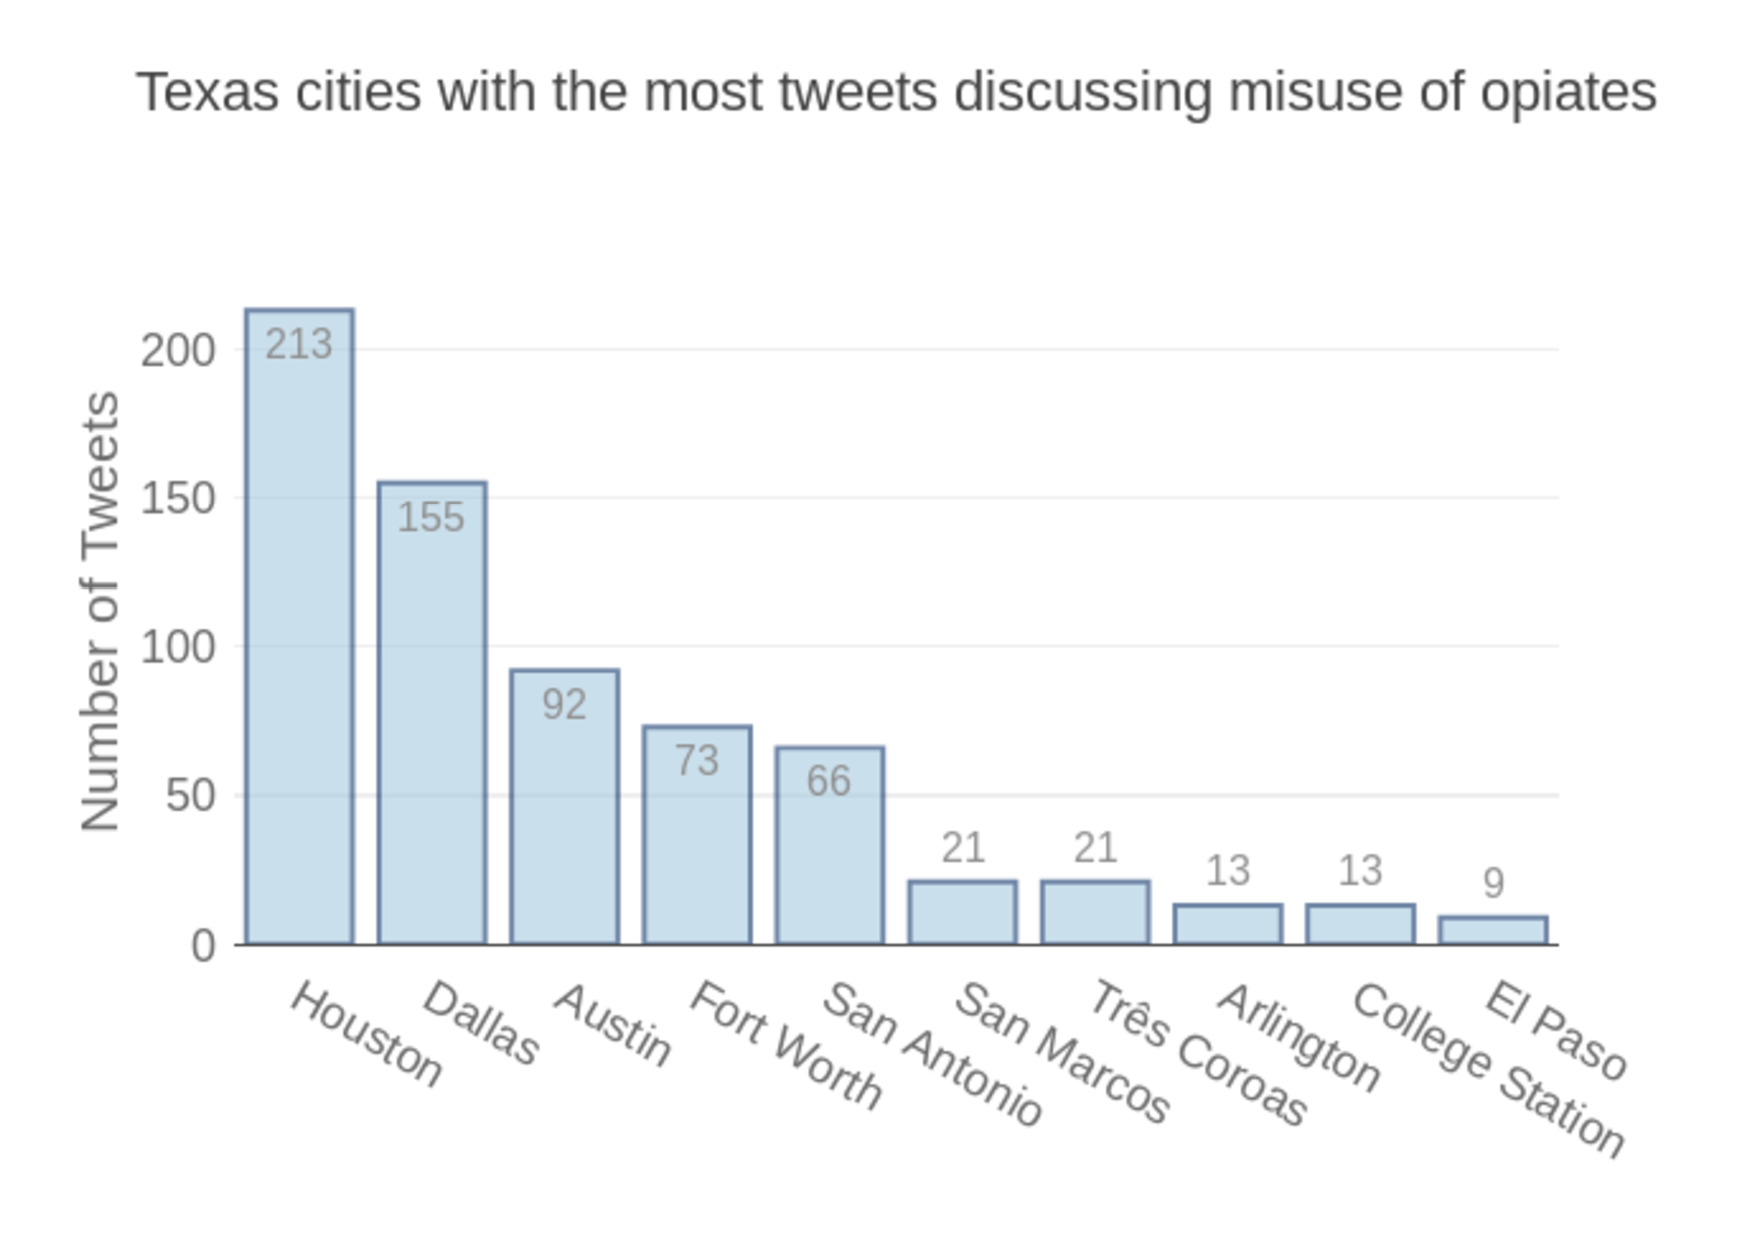
\includegraphics[width=\columnwidth]{images/Figure1.pdf}
  \caption{Number of Tweets by Population (per 100,000)}
  \label{f:Figure1}
\end{figure}

\begin{figure}[!ht]
  \centering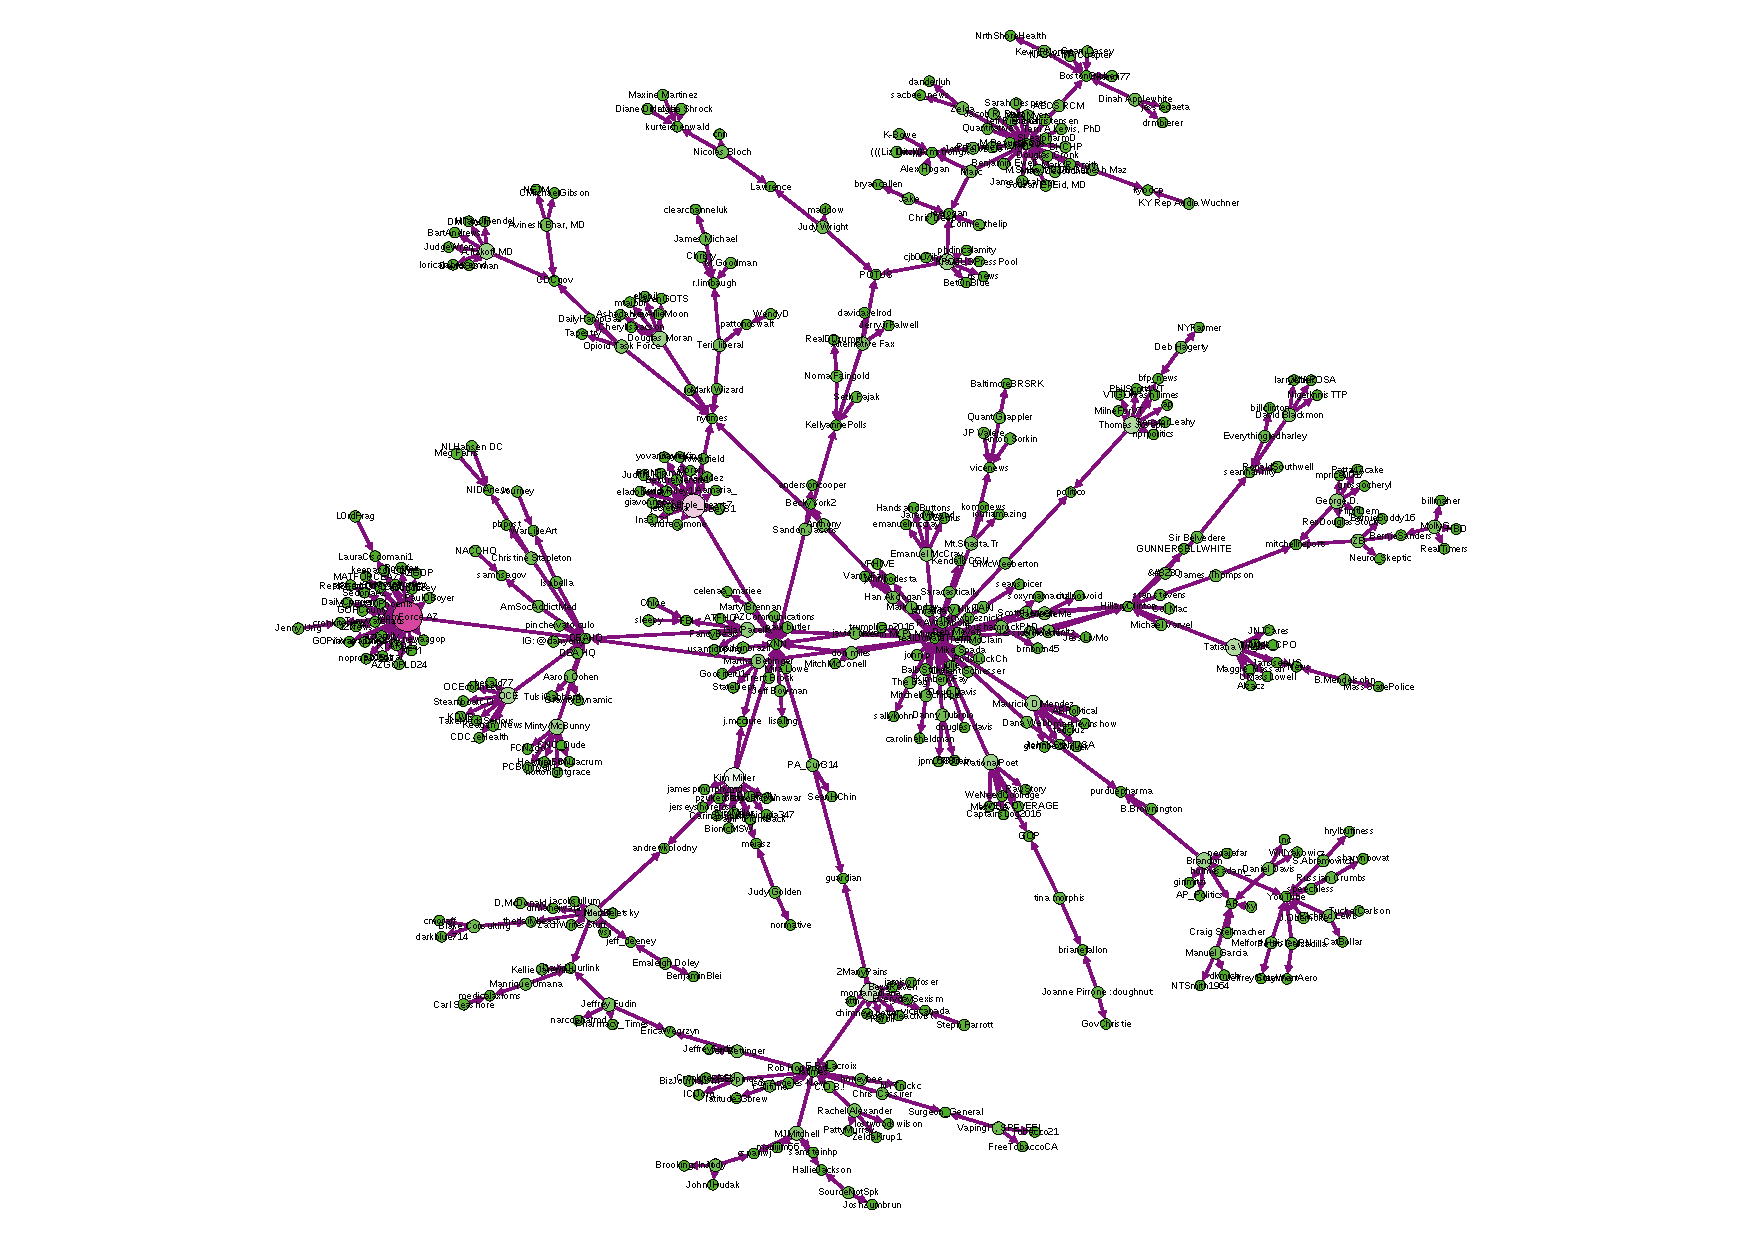
\includegraphics[width=\columnwidth]{images/Figure2.pdf}
  \caption{Number of Tweets by Tweet Volume (per 100,000)}
  \label{f:Figure2}
\end{figure}

Figure 1 and Figure 2 show state baseline data of ``tweet volume'' in contrast 
to ``tweet count'' the number of opiate-referring tweets we collected for each 
state in this study. Table 4 shows the data by normalizing state tweet counts 
on population. The same data (`Tweetstats.csv') was used as in input for these 
charts. (Note: Interactive features of the Figures are not enabled in the 
\emph{LaTex} document). As Figure 1 shows, Georgia has highest number of opiate-
related tweet per 100 thousand tweets (tweet volume). Texas followed by 
California are at second and third position regarding the number of opiates 
related tweets as compared to the tweets volume. In New York, the number of 
opiate-related tweets out of the tweets volume was lowest. Figure 2 shows number 
of tweets with respect to the population of state. It is not surprising that the 
second most populous state Texas has the highest number of opiates-related tweets 
per 100 thousand people. However, Georgia with least population has second highest 
number of opiate-related tweets is quite surprising. Source code for these 
charts is provided in an interactive notebook \emph{TweetsStatistics.ipynb}. 

\begin{figure}[!ht]
  \centering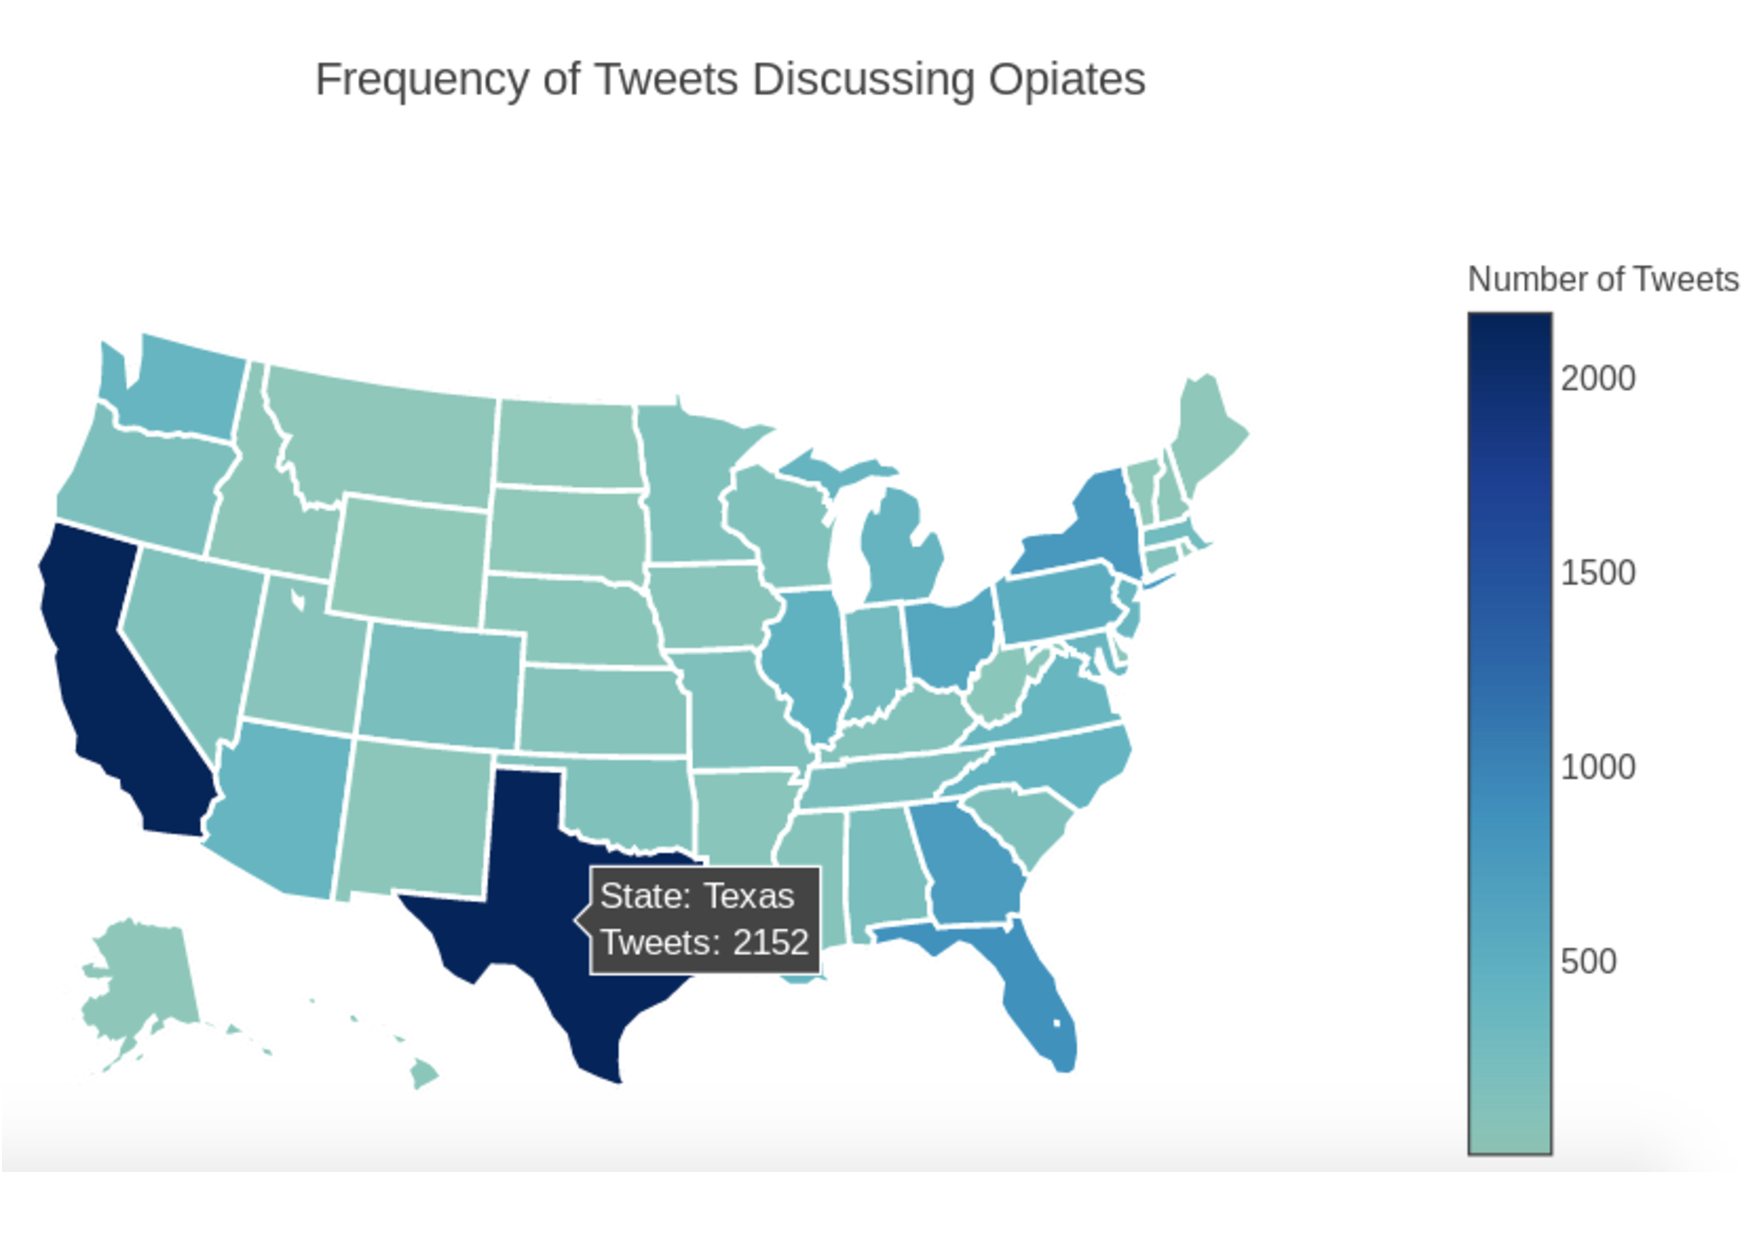
\includegraphics[width=\columnwidth]{images/Figure3.pdf}
  \caption{Choropleth Map of Opiate Tweet Frequency in U.S.}
  \label{f:Figure3}
\end{figure}

\begin{figure}[!ht]
  \centering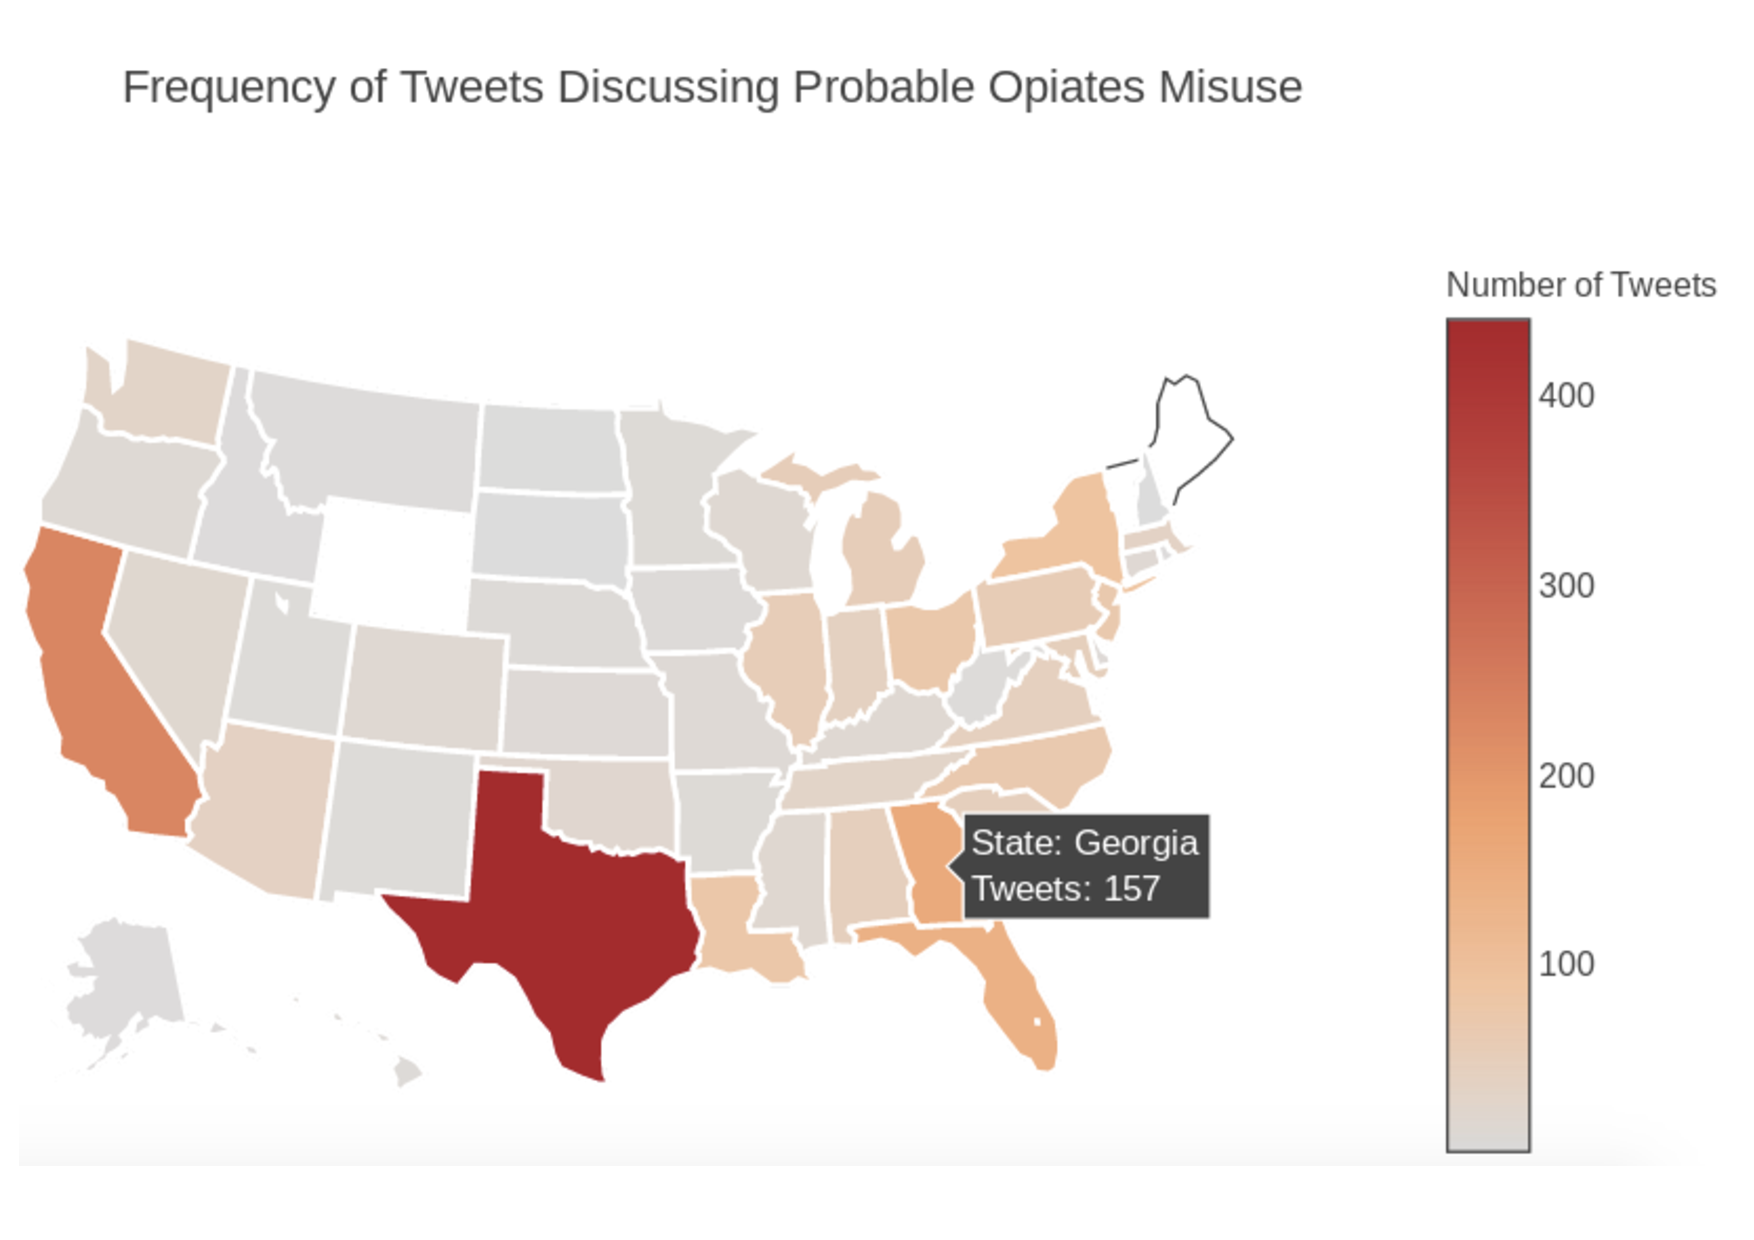
\includegraphics[width=\columnwidth]{images/Figure4.pdf}
  \caption{Choropleth Map of Probable MUPO Tweet Frequency in U.S.}
  \label{f:Figure4}
\end{figure}

The MUPO tweet data was plotted on two different U.S. state maps. Figure 3 
shows the locations and frequency of all the users tweeting about opioids. 
Figure 4 shows the frequency of tweets discussing probable misuse of opioids. 
Data from `FinalTweets.csv' is used for these geospatial maps. Figure 3 shows 
the state-wide distribution of opiates related tweets. The color scale from 
dark blue to faint blue shows the highest to lowest tweet frequency. Analysis 
shows that California and Texas are the states tweeting about opiates the most, 
followed by Florida and New York. In an interactive version of this plot, a 
mouse hover over the plot shows the name of state and total number of tweets. 
State-wise distribution in Figure 4 shows California and Texas tweeting the 
most about probable opioids misuse. MUPO tweet data of these two states is 
further sliced down to show top ten cities with the highest frequency of 
opiate-related tweets (Figure 5 and Figure 6). Los Angeles and Houston top 
the list in their respective states for highest MUPO-related tweets. 

\begin{figure}[!ht]
  \centering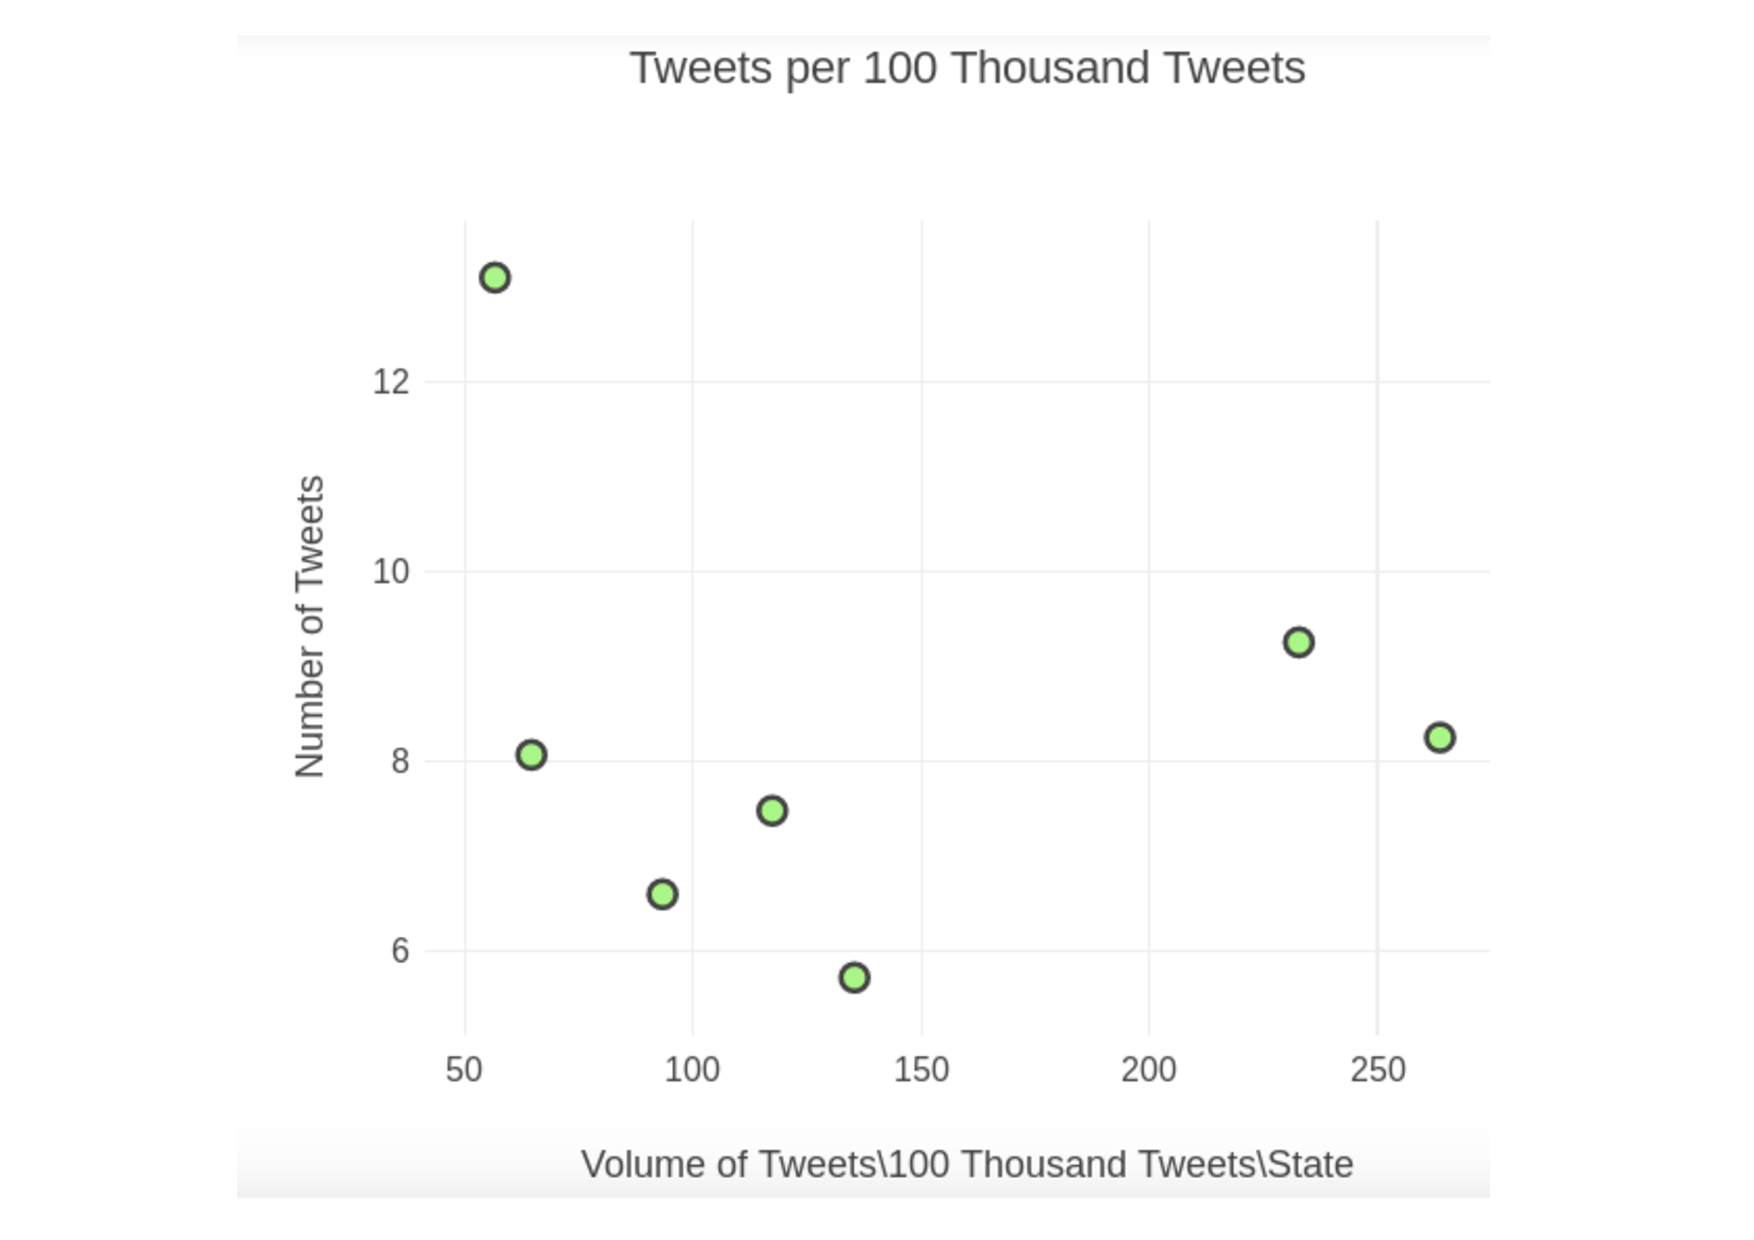
\includegraphics[width=\columnwidth]{images/Figure6.pdf}
  \caption{California Cities with the Most Tweets Discussing 
  Misuse of Opiates}
  \label{f:Figure5}
\end{figure}

\begin{figure}[!ht]
  \centering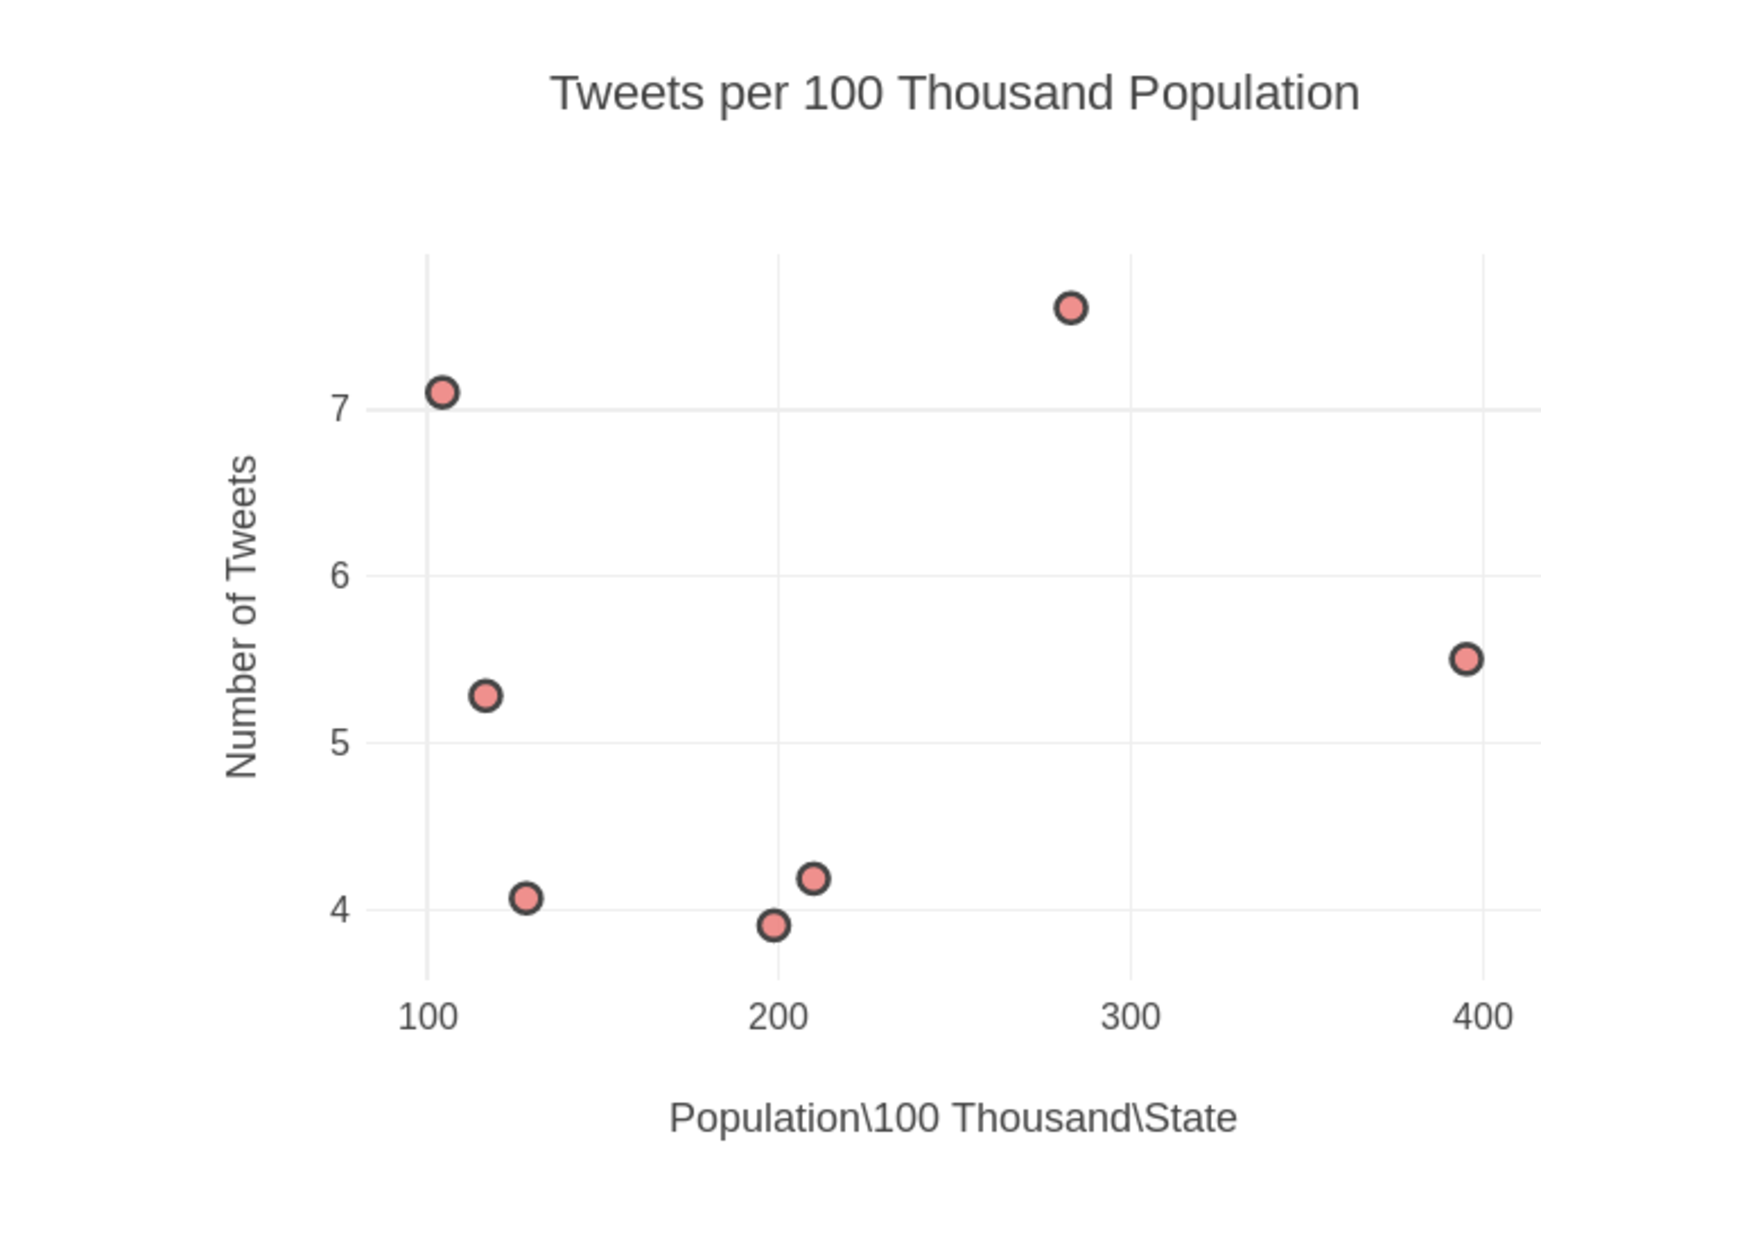
\includegraphics[width=\columnwidth]{images/Figure5.pdf}
  \caption{Texas Cities with the Most Tweets Discussing Misuse of Opiates}
  \label{f:Figure6}
\end{figure}


%%%%%%%%%%%%%%%%%%%%%%%%%%%%%%%%%%%%%%%%%%%%%%%%%%%%%%%%%%%%%%%%%%%%%%%%%%%%%%%%

\subsection{Network Analysis} 

This section examines the network of connections among Twitter users sharing 
mentions about the misuse of prescription opioids. The network analysis and 
creation of the adjacency matrix were implemented in an interactive Python 
notebook (\emph{SMM-Project-TweetMatcher-Mentions.ipynb}). An initial network 
was constructed from a data set of 16,964 tweets with 17 features (in CSV 
format, saved as a pickle file: `SMM-cleanedTweets-16964.pkl'). The data set 
was opened in Pandas and saved as a data frame object that was filtered to 
select only tweets that included mentions, which returned 3176 tweets. An 
adjacency matrix was created by pairing `userName' and tweet `txt' as a list 
of tuples using the zip method. A function called `TweetMatcher()` was used 
to iterate through the list of tweet, and extract the user name and mention 
included in each text, and append them in a separate line of a new list called 
‘myMentions’, that consisted of 4598 `userName'-`mention' pairs. The adjacency 
matrix was used to create a directed graph (DiGraph) in \ephm{NetworkX}. 
The network graph was written to .gml file and imported into \emph{Gephi} for 
visualization. The resulting network consisted of 6091 nodes and 4105 edges. 
The average out degree was 0.674, network diameter was 1, the modularity 
coefficient was 0.994, with 2011 components, and an average path length of 1. 
The nodes were ranked by color and size according to out-degree, and the 
Yifan Hu algorithm was used to orient the graph layout.

\begin{figure}[!ht]
  \centering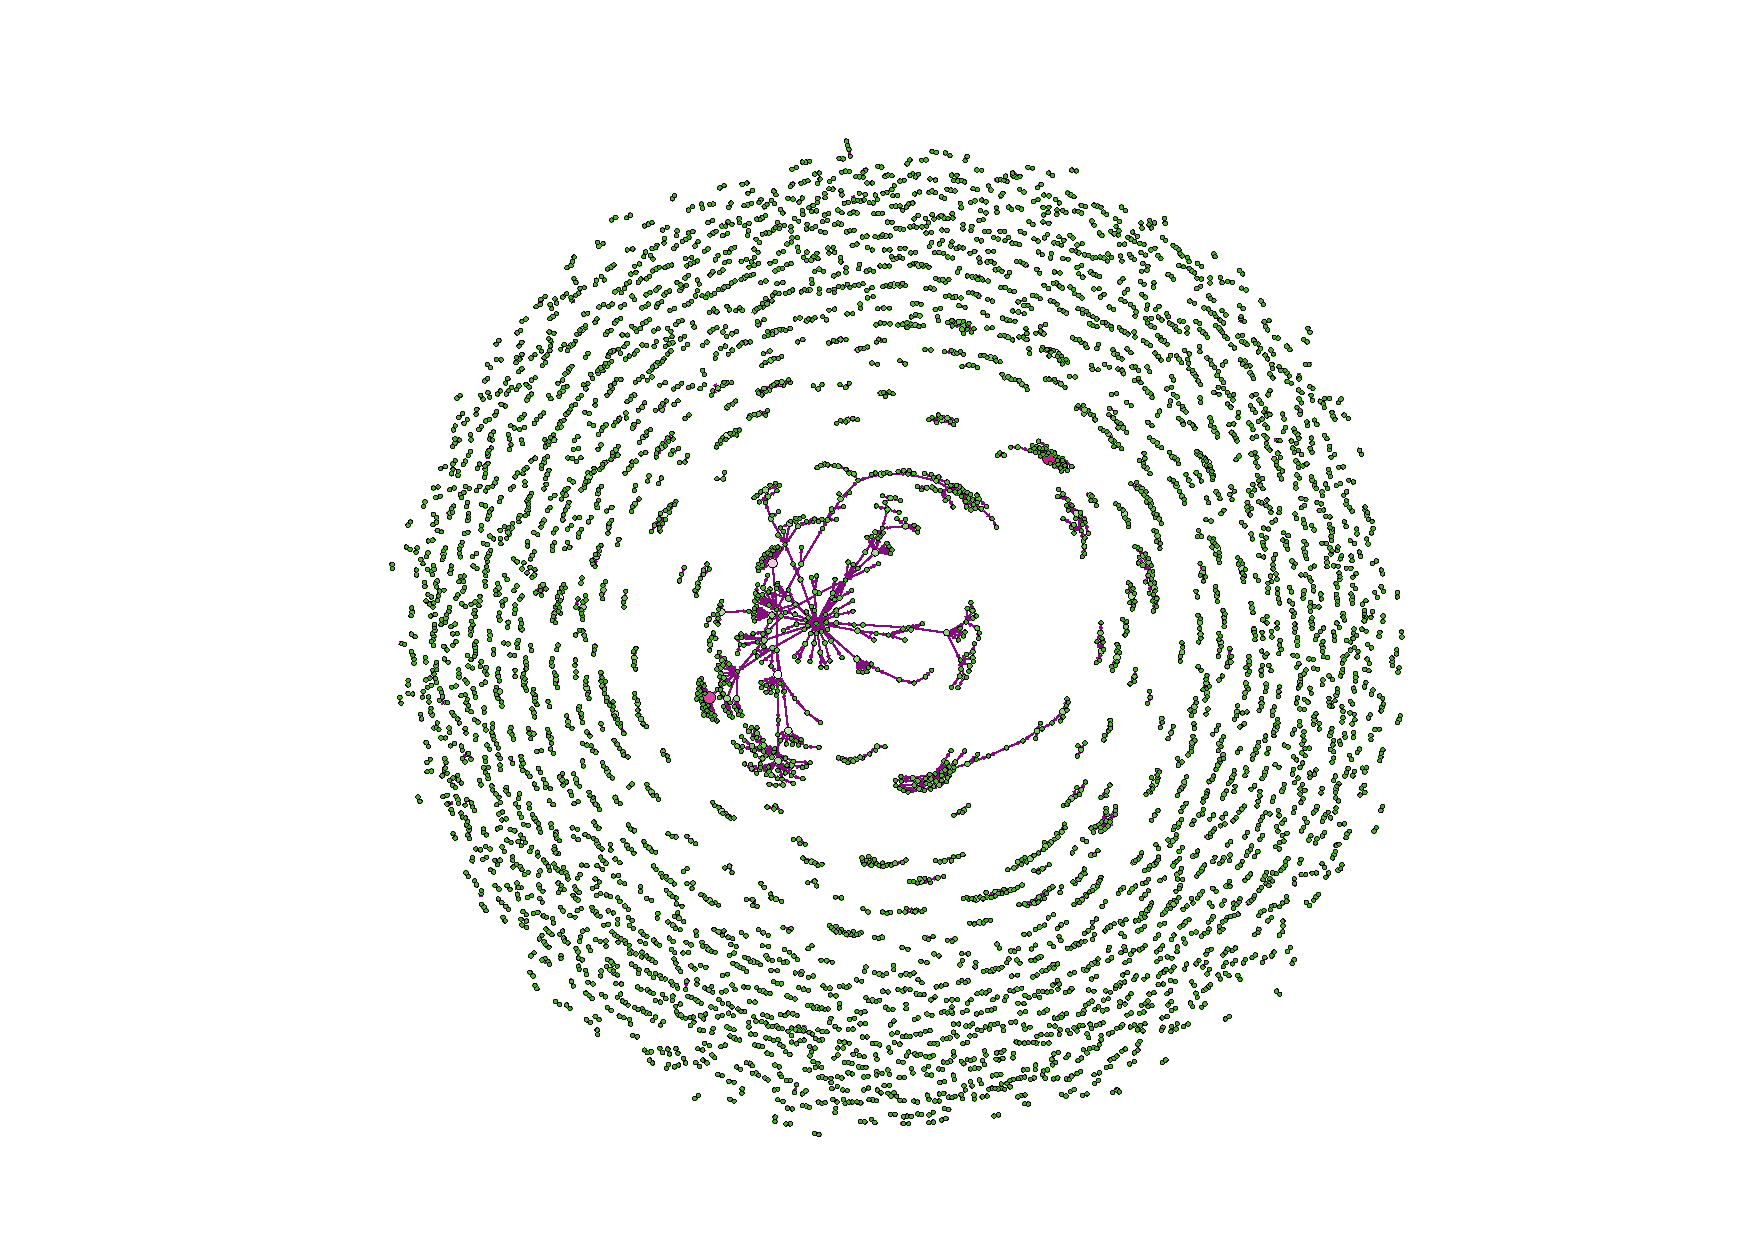
\includegraphics[width=\columnwidth]{images/Figure7.pdf}
  \caption{Network of Twitter Mentions Related to Misuse of Prescription 
  Opioids (MUPO)}
  \label{f:Figure7}
\end{figure}

Figure 7 shows the full directed network of tweet mentions related to misuse
of prescription opioids (MUPO). As figure 7 shows, the graph consists of a 
large number of low degree nodes with only one or two mentions, and a small 
number of nodes with a larger number of mentions; however, the graph does 
not possess small-world properties as it consists of largely disconnected 
nodes, with a connected component toward the center of the graph. Initially, 
it was hypothesized that the social network of Twitter user MUPO mentions 
would have several connected components based on different aspects of opioid use.  
To examine connections among user mentions, the network was filtered using
\emph{Gephi} to select the largest giant component, which is shown in Figure 8. 
The giant filtered component consisted of 454 nodes (7.5 \%) and 462 edges 
(11.25 \%). The giant component displayed in Figure 8 shows a small number of 
users with an out-degree greater than 10, and a small number of nodes with 
in-degree greater than 10. Given that the edges are directed, the ``hubs'' with 
large out-degree do not form bridges between different components. What we
see instead suggests several disconnected conversations directed in different
directions. Although a small number of mentions are directed at legitimate 
agencies related to opioid addiction and the opioid crisis (e.g., CDCgov, 
CDC-eHealth, Opioid Task Force, NIDA-news), a large number of mentions were 
directed at political candidates (e.g., realDonaldTrump, HillaryClinton) or
news outlets (BostonGlobe, CNN, NYTimes, LATimes, ViceNews). 

\begin{figure}[!ht]
  \centering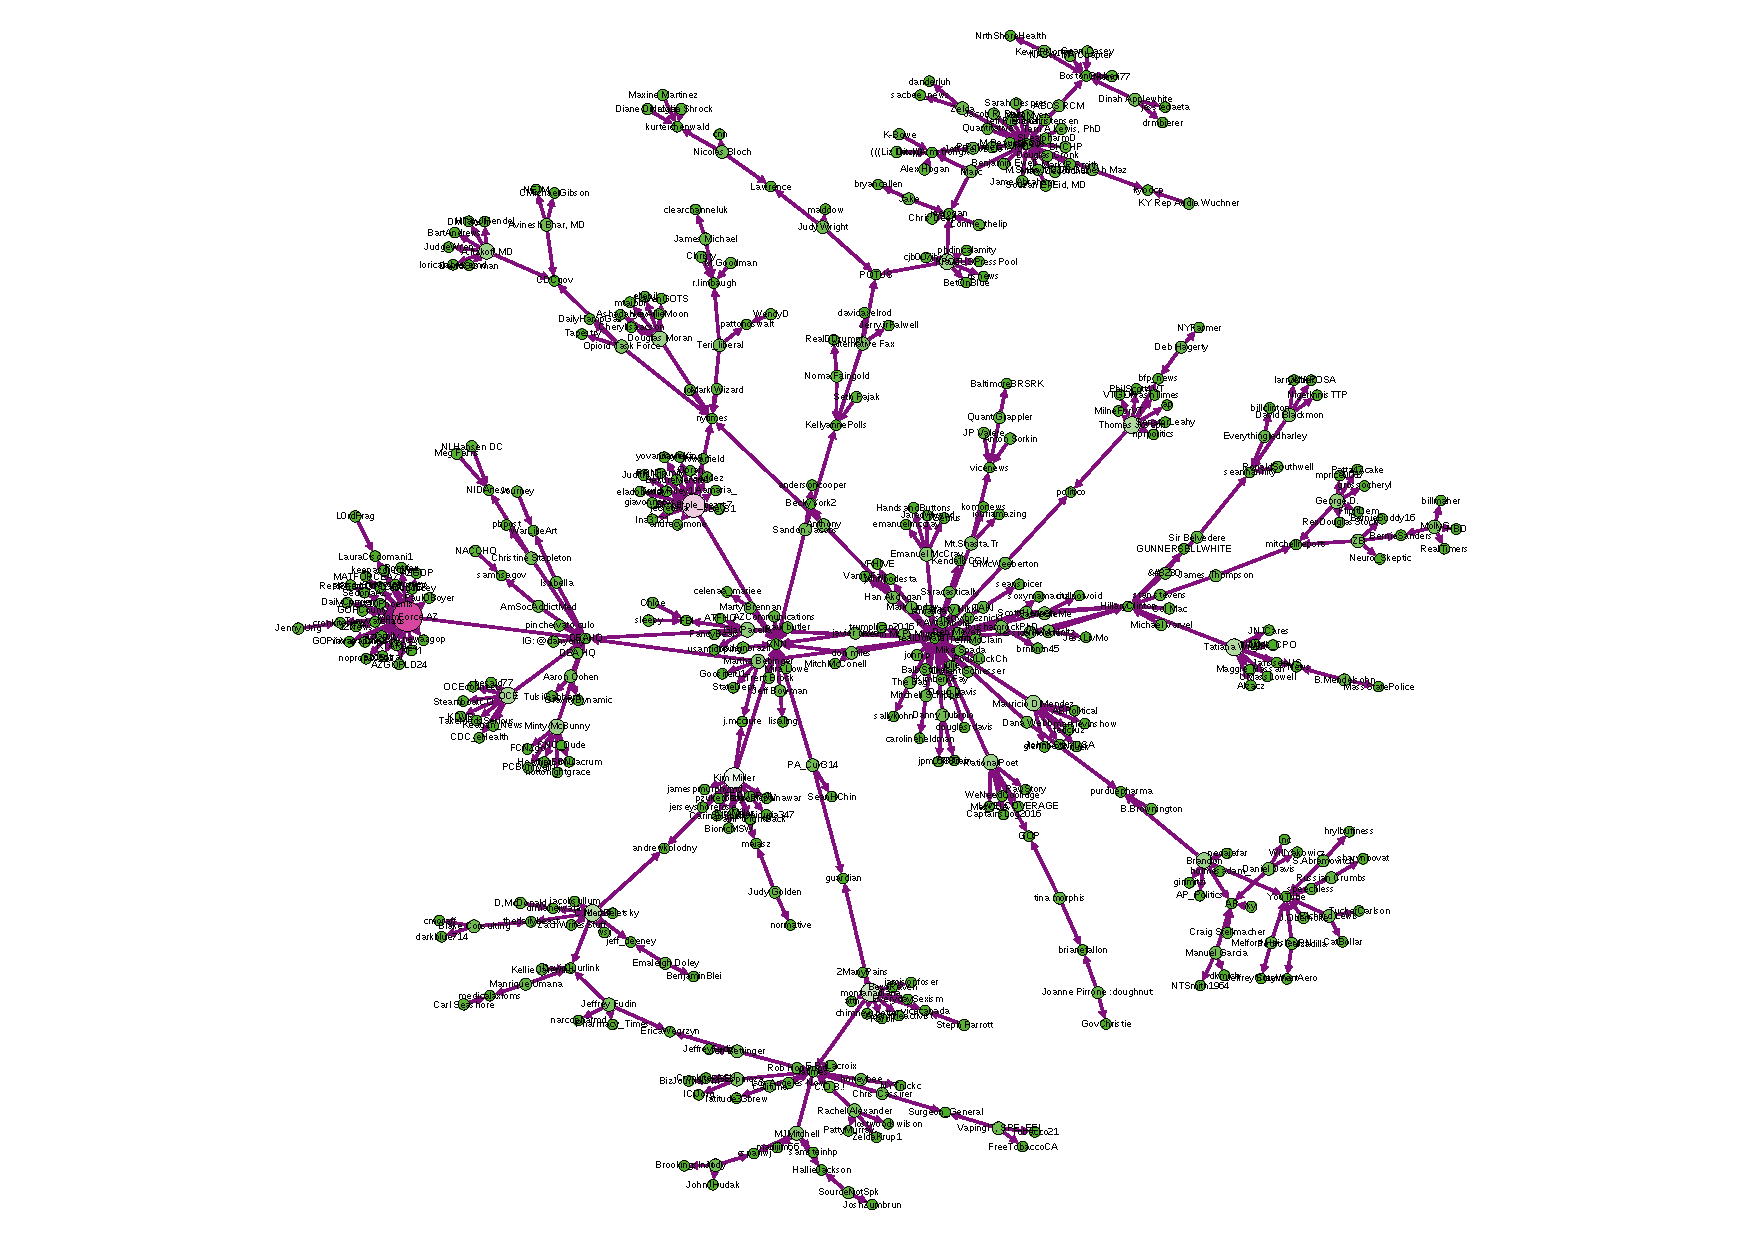
\includegraphics[width=\columnwidth]{images/Figure8.pdf}
  \caption{Largest Component of the Network of Twitter Mentions Related to 
  Misuse of Prescription Opioids (MUPO)}
  \label{f:Figure8}
\end{figure}

Additional data cleaning was performed based on a classification of tweets
with MUPO versus non-MUPO content (described above), resulting in a final data 
set of 15,247 tweets. From this final data set, 2127 (14\% of total) were 
classified as actual MUPO related content, 93 (4\% of subset) included mentions. 
An additional 29 tweets were identified as deriving from rap song lyrics and 
removed. A third network was constructed from the adjacency matrix for 64 MUPO 
tweets with mentions (`smm-misuseTweets-mentions.csv'). The graph was created 
using \emph{NetworkX}, written to .gml file, and imported to \emph{Gephi} for 
visualization. The resulting network consisted of 131 nodes with 71 edges, with 
an average out-degree of 0.542; the modularity coefficient was 0.981, and the 
graph had 60 components. The Fruchterman-Reingold algorithm was selected to 
orient the graph layout. The graph represented in Figure 9 shows a large number 
of nodes with only a single out-degree, and a small number of nodes with an 
out-degree of 2 or 3. The graph no longer had a connected component. This 
reduced directed network consisted largely of many disconnected nodes, each 
with only a small number of mentions; unfortunately this graph did not support 
analysis of the network flow, centrality, or community structure 
\cite{golbeck13, zafarani14}. Although some tweets were directed at legitimate 
agencies such as the Department of Veteran Affairs), there were some mentions 
in the MUPO tweets directed at celebrity figures from popular culture or 
pseudonyms (e.g., ``Eminem'', ``Hulk Hogan'', ``real dope celebrity''). 

\begin{figure}[!ht]
  \centering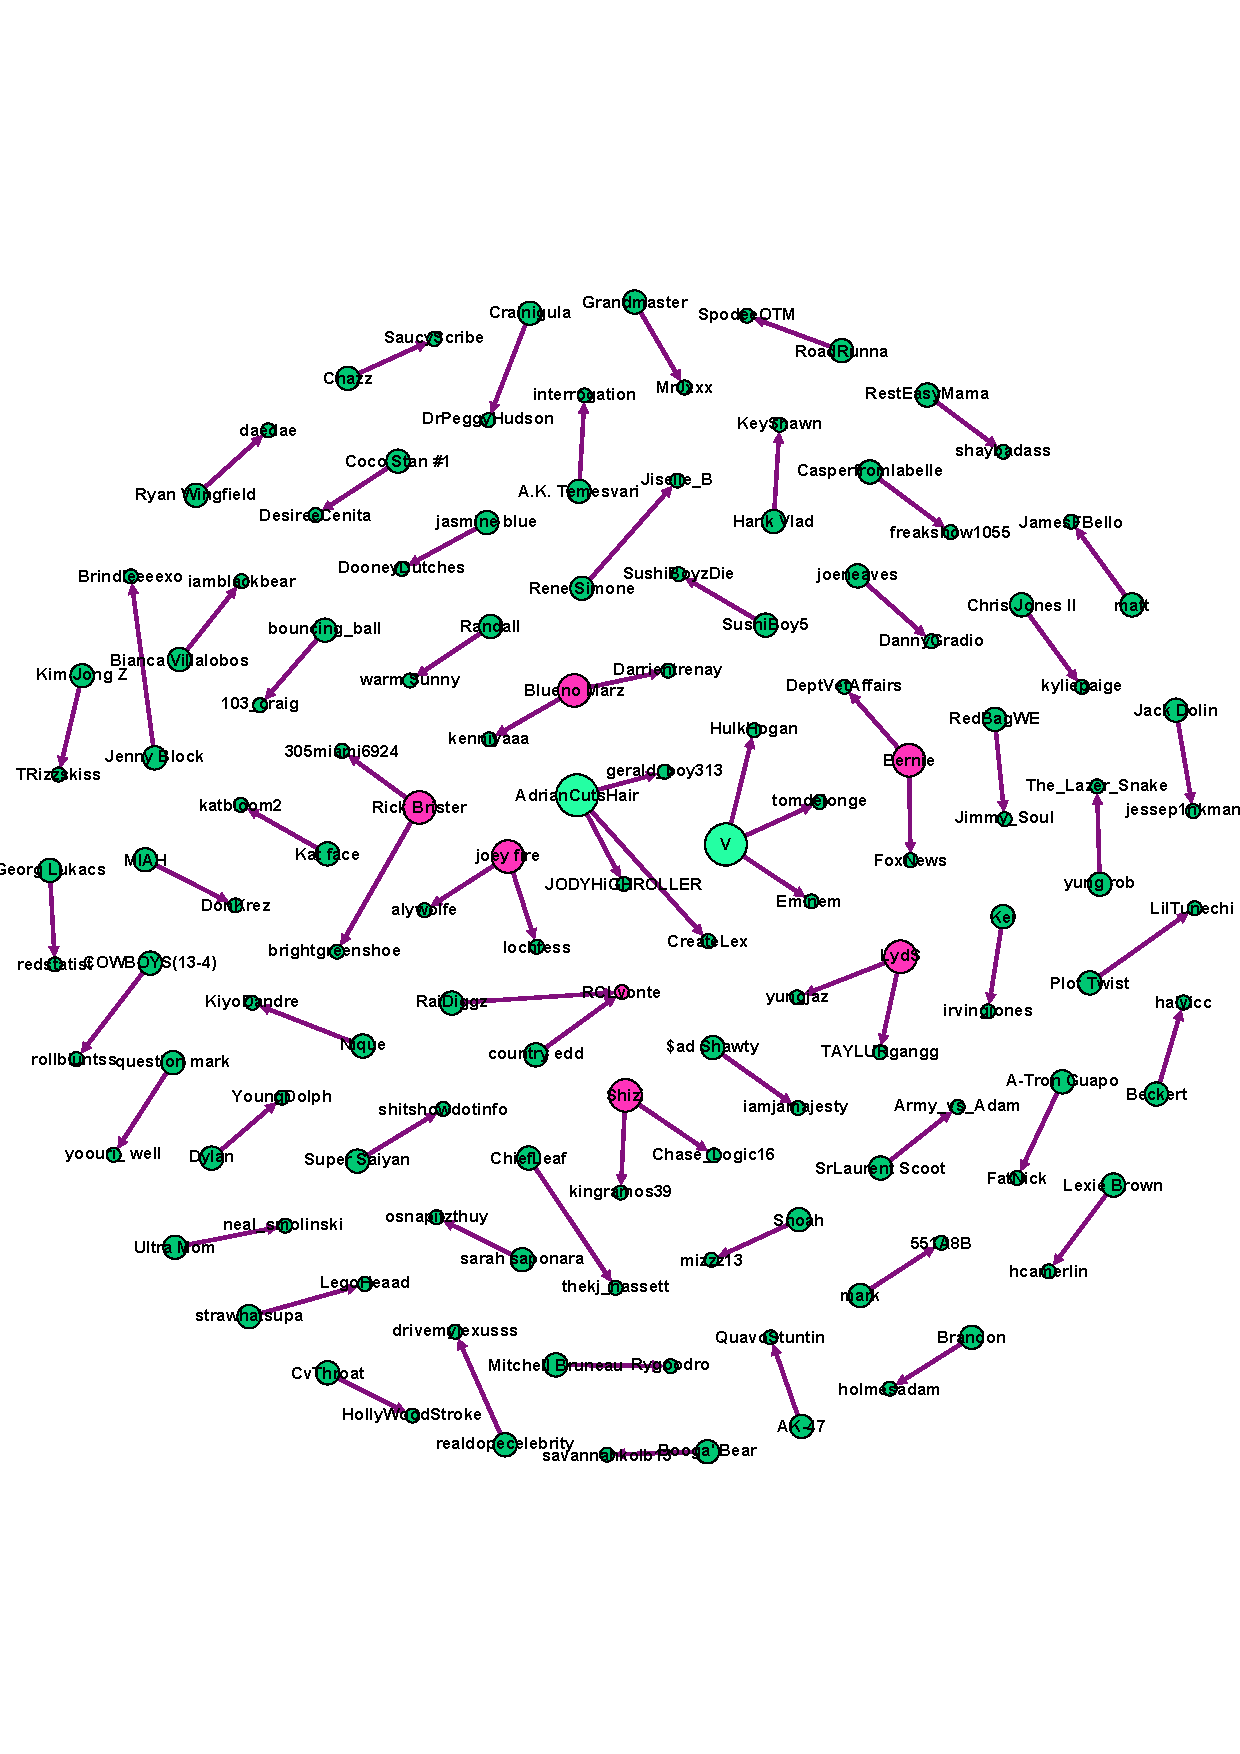
\includegraphics[width=\columnwidth]{images/Figure9.pdf}
  \caption{Directed Network of MUPO Twitter User Mentions}
  \label{f:Figure9}
\end{figure}

%%%%%%%%%%%%%%%%%%%%%%%%%%%%%%%%%%%%%%%%%%%%%%%%%%%%%%%%%%%%%%%%%%%%%%%%%%%%%%%%
\section{Discussion}

This project applied the tools of infodemiology in social media to explore the 
misuse of prescription opioids (MUPO) and map the relations among Twitter 
users discussing MUPO online. We integrated several approaches to better 
understand what social media can tell us about the structure of interaction on 
Twitter related to MUPO. Textual analysis and classification of tweets revealed 
that approximately 14\% of the tweets in our sample contained MUPO content. 
Several iterations of data cleaning were required to obtain a data set that 
filtered out non-MUPO tweets and mentions. Geospatial analysis revealed that 
California and Texas emerged as topmost states to tweet about probable misuse
of opioids. Although these are the two most populous states, the frequency of 
opiate-related tweets was not directly proportional to population. For example, 
the tweet count per 100 thousand population was higher for Georgia than 
California. Similarly, despite the state of New York having a large population, 
the tweet count ratio per 100 thousand population for New York was lower than 
for Georgia. Analysis of mentions among Twitter users discussing MUPO revealed 
a highly disconnected network with a large number of nodes with low out-degree, 
and few users sharing MUPO mentions with more than two or three other users. 
Examining mentions about opioids more broadly revealed a central component of 
users sharing mentions about opioids with ten or more other users, and a 
handful of users receiving more than 10 mentions from others. Counter to 
our hypothesis, this largely disconnected network did not reveal underlying 
community structure or connections between separate components. 

%%%%%%%%%%%%%%%%%%%%%%%%%%%%%%%%%%%%%%%%%%%%%%%%%%%%%%%%%%%%%%%%%%%%%%%%%%%%%%%%

The first question we proposed to answer in this project is whether opioid 
misuse could be detected from Twitter posts. We looked to past studies that 
examined how social media data was used to forecast outbreaks of flu 
\cite{culotta10, paul14}, or how tweets could predict geographic variation 
in opioid misuse \cite{chary17, sarker16}. Although we were able to classify 
MUPO tweets from non-MUPO tweets using supervised learning models, several 
iterations of data cleaning and filtering reduced our sample of Twitter data
which may have limited the usefulness of the remaining tweets for ascertaining
the genuineness of actual instances of MUPO. Second, we were able to map
the frequency of opiate-related tweets by geographic location at the level 
of state and U.S. cities; however, as described above the frequency of tweets
by population may not correspond with the actual rates of MUPO by region or 
tweet volume. Third, we sought to identify the relationships among Twitter 
users discussing opioid misuse by their mentions, but found a vastly reduced 
and disconnected network that lacked community structure. Despite an ambitious 
effort on our part, overall, we encountered some ambiguity in being able to 
identify actual opioid misuse, mapping the occurrence of actual misuse from 
tweet location, and visualizing the social network of relations among twitter 
users who may be misusing opioids.

%%%%%%%%%%%%%%%%%%%%%%%%%%%%%%%%%%%%%%%%%%%%%%%%%%%%%%%%%%%%%%%%%%%%%%%%%%%%%%%%

\subsection{Limitations}

Our project had some limitations. First, in examining the MUPO-related tweets 
and mentions, we encountered numerous instances of opioid misuse from music and 
popular culture, that were non-MUPO but labeled as MUPO. Twitter data suffers 
from a common problem encountered with self-report data in the social sciences, 
namely, people are not always honest in how they represent themselves in surveys
or online. For example, people tend to exaggerate behavior they perceive as 
desirable and minimize behaviors perceived as undesirable. In youth culture, 
this often involves adhering to the norms of a subculture by pretending to be 
``cool'' or pretending to be ``clean''. Tweets with MUPO-content from song 
lyrics may reflect some sentiment elsewhere or overall in the song, could
reflect actual substance use, or an indicator for membership in a subculture; 
the opoid-included lyric is simply the most recognizable short reference. 
Another limitation is that, we created successive subsets of the data  initially 
extracted from Twitter, for the sake of consistency. Given that geospatial 
mapping was a central goal of our project, by necessity, we extracted tweets 
that included latitude and longitude, where generally only a small proportion 
of tweets (1\%-2\%) includes geospatial information. Selecting tweets with 
mentions from the subset of tweets with geolocation reduced the sample of 
tweets for network analysis. In future research, it might be desirable to 
extract separate samples of tweets with geospatial location and tweets with 
mentions for network analysis, for more robust samples in each analysis. 

%%%%%%%%%%%%%%%%%%%%%%%%%%%%%%%%%%%%%%%%%%%%%%%%%%%%%%%%%%%%%%%%%%%%%%%%%%%%%%%%
\section{Conclusion}

The misuse and abuse of opioids remains a serious health crisis affecting 
millions of people in North America. Given the scale of the opioid misuse, 
abuse, and addition, addressing the opioid crisis will require large scale 
efforts and interdisciplinary interventions that are well beyond the scope 
of our project. This project may help to raise awareness of MUPO on social
media by identifying MUPO-related posts on Twitter, mapping the locations of 
potential or probable MUPO, and visualizing relations among user discussing 
MUPO on Twitter. Mapping social media content related to MUPO may not only
help detect individuals at risk for opioid misuse, abuse, or addiction, 
but network analysis may help to identify communities and subcultures in 
which MUPO is regarded as more acceptable, such as was observed in references
to music lyrics and popular culture. Different communities may be responding
to MUPO in different ways, either popularizing or romantisizing opiate use, 
or by addressing the crisis with treatment and interventions, sharing 
information and references for rehab and detoxification. Given that many 
patients legitimately prescribed opioids for chronic pain transition to 
heroin and are at risk for opioid overdose and deaåth, social media may help
to track instances of MUPO and provide an early warning system for MUPO 
hotspots. Understanding the network of relations of åusers in social media
discussing MUPO may provide insight as to how to address the crisis of 
opioid abuse and addiction from a novel perspective. 
 
%%%%%%%%%%%%%%%%%%%%%%%%%%%%%%%%%%%%%%%%%%%%%%%%%%%%%%%%%%%%%%%%%%%%%%%%%%%%%%%%

\section{Contributions}

All team members contributed approximately equally to writing the research 
proposal and report. Elizabeth Supinski extracted the data from the Twitter 
API, performed data cleaning and preparation, annotated tweet text, ran the 
classification models of tweets for MUPO content, and created the Tables. 
Nandita Sathe set up and explored the use of \emph{Carmen} for geolocating 
tweets, constructed Geospatial plots and maps (Figures 1-6), and set up of 
BitBucket for project source collaboration. Sean Shiverick conducted the 
network analysis, constructed the adjacency matrix and network graph, 
created network visualizations in \emph{Gephi} (Figures 7-9), and formatted 
the project proposal and report in ACM Proceedings format in \emph{Sharelatex}.

\begin{acks}
  The authors would like to thank Dr. Vincent Malic and J. T. Wolohan 
  for support and assistance in the completion of this project, and to 
  the reviewers who provided feedback on the project proposal.
\end{acks}

\bibliographystyle{unsrt}
\bibliography{report} 

%%%%%%%%%%%%%%%%%%%%%%%%%%%%%%%%%%%%%%%%%%%%%%%%%%%%%%%%%%%%%%%%%%%%%%%%%%%%%%%%

\appendix

\section{Appendix A: Tweets Proportional to Population}
The Table below provides a summary of Tweets Proportional to Tweet 
Volume and Population, as described in the Classification subsection of 
the Data Description section.

\begin{table*}[ht]
\centering
\caption{Tweets Proportional to Tweet Volume and Population}
\label{tab:1}
  \begin{tabular}{lllllll}
    \toprule
    State & Tweet Count & Population & (A) Opiate tweets/100k & Tweet Volume & 
    (B) Opiate tweets/100k & Ratio B/A \\
    \midrule     
    CA& 2176& 39,540,000& 5.50& 26,374,150& 8.25& 1.5 \\
    TX& 2154& 28,300,000& 7.61& 23,279,069& 9.25& 1.22 \\
    FL& 878& 20,980,000& 4.18& 11,737,449& 7.48& 1.79 \\
    NY& 775& 19,850,000& 3.9& 13,538,927& 5.72& 1.47 \\
    GA& 741& 10,430,000& 7.1& 5,660,441& 13.09& 1.84 \\
    OH& 616& 11,660,000& 5.28& 9,331,571& 6.60 & 1.25 \\
    PA& 521& 12,810,000& 4.07& 6,457,351& 8.07& 1.98 \\	
    \bottomrule
  \end{tabular}
\end{table*}





%\input{issues}

\end{document}
